\hypertarget{zbiornik_8cpp}{\section{Dokumentacja pliku zbiornik.\-cpp}
\label{zbiornik_8cpp}\index{zbiornik.\-cpp@{zbiornik.\-cpp}}
}


Zawiera definicje metod klasy \hyperlink{class_zbiornik}{Zbiornik}.  


{\ttfamily \#include \char`\"{}zbiornik.\-hh\char`\"{}}\\*
Wykres zależności załączania dla zbiornik.\-cpp\-:
\nopagebreak
\begin{figure}[H]
\begin{center}
\leavevmode
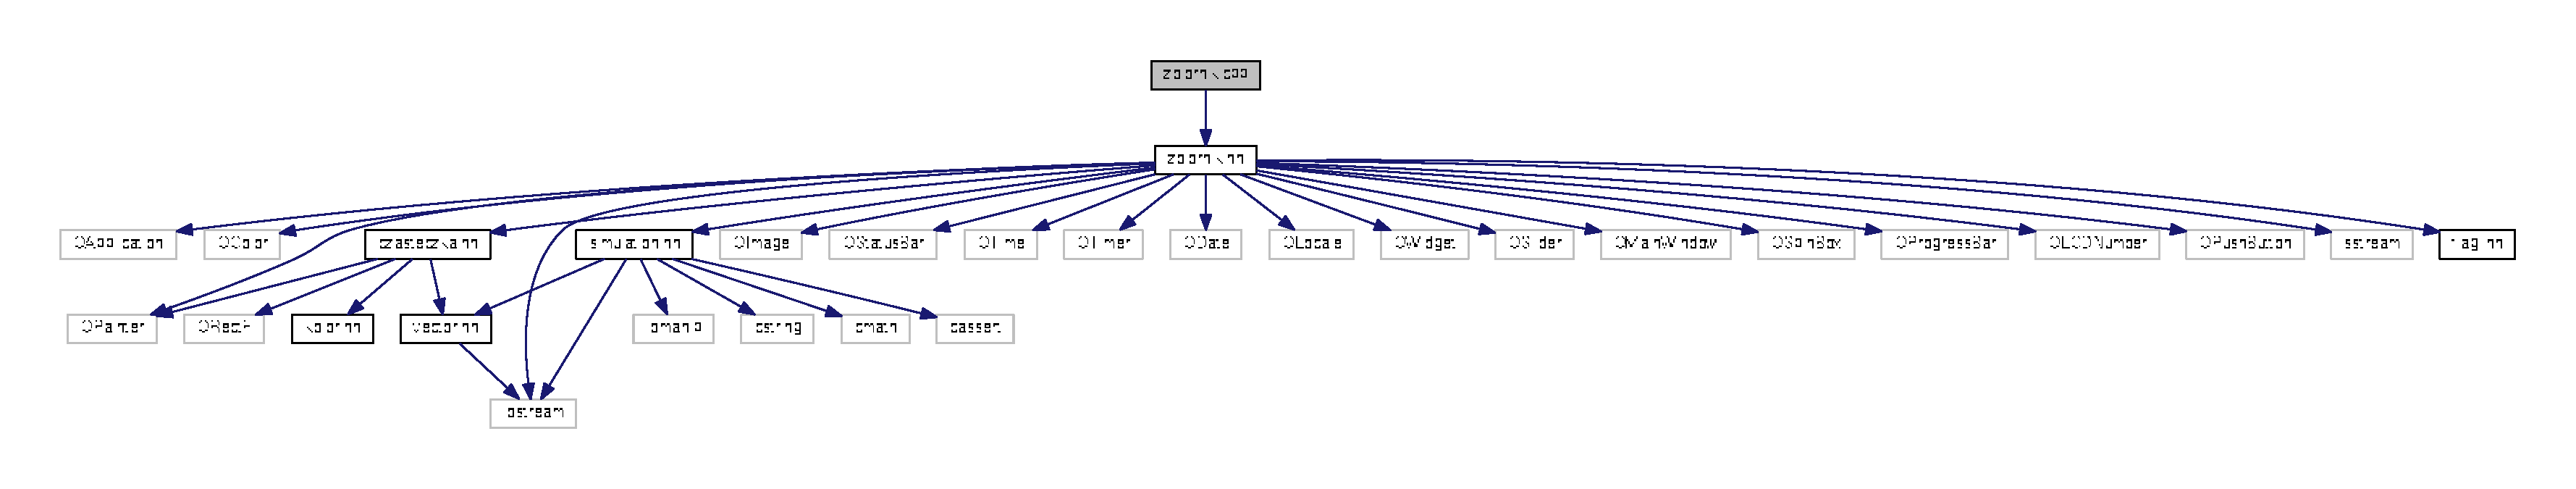
\includegraphics[width=350pt]{zbiornik_8cpp__incl}
\end{center}
\end{figure}


\subsection{Opis szczegółowy}
W pliku znajduja sie\-:
\begin{DoxyItemize}
\item definicje konstruktorow, metod i przeciazen klasy \hyperlink{class_zbiornik}{Zbiornik}. 
\end{DoxyItemize}

Definicja w pliku \hyperlink{zbiornik_8cpp_source}{zbiornik.\-cpp}.

